\chapter{Functions and Derived Distributions}
\index{Functions of Random Variables}

We already know from our previous discussion that it is possible to form new discrete random variables by applying real-valued functions to existing random variables.
In a similar manner, it is possible to generate a new random variable $Y$ by taking a well-behaved function $g(\cdot)$ of a continuous random variable $X$.
The graphical interpretation of this notion is analog to the discrete case and appears in Figure~\ref{figure:FunctionContinuousRV}.

\begin{figure}[ht]
\begin{center}
\begin{psfrags}
\psfrag{S}[l]{Sample Space}
\psfrag{X}[c]{$X$}
\psfrag{Y}[c]{$Y = g(X)$}
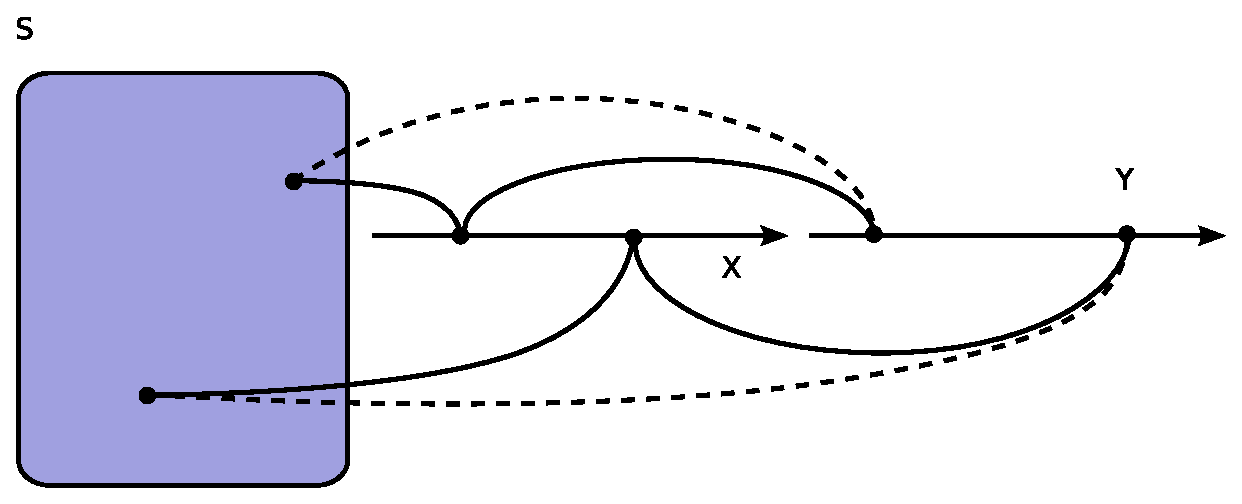
\includegraphics[width=9.26cm]{Figures/9Chapter/fcn-cnt}
\end{psfrags}
\caption{A function of a random variable is a random variable itself.
In this figure, $Y$ is obtained by applying function $g(\cdot)$ to the value of continuous random variable $X$.}
\label{figure:FunctionContinuousRV}
\end{center}
\end{figure}

Let $X$ be a continuous random variable, and let $g: \RealNumbers \mapsto \RealNumbers$ be an admissible function.
Variable $Y = g(X)$, defined pointwise, is itself random.
The probability that $Y$ falls in a specific set $S$ depends on both the function $g(\cdot)$ and the PDF of $X$,
\begin{equation*}
\Pr (Y \in S) = \Pr (g(X) \in S) 
= \Pr \left( X \in g^{-1}(S) \right)
= \int_{g^{-1} (S)} f_X (\xi) d\xi .
\end{equation*}
In particular, we can derive the CDF of $Y$ using the formula
\begin{equation} \label{equation:DerivedCDF}
F_Y(y) = \Pr (g(X) \leq y)
= \int_{ \{ \xi \in X(\Omega) | g(\xi) \leq y \} } f_X(\xi) d\xi .
\end{equation}

\begin{example}
Let $X$ be a Rayleigh  random variable with parameter $\sigma^2  = 1$, and define $Y = X^2$.
We wish to find the distribution of $Y$.
From \eqref{equation:DerivedCDF}, we can compute the CDF of $Y$.
For $y > 0$, we get
\begin{equation*}
\begin{split}
F_Y(y) &= \Pr (Y \leq y) = \Pr \left( X^2 \leq y \right) \\
&= \Pr (- \sqrt{y} \leq X \leq \sqrt{y})
= \int_0^{\sqrt{y}} \xi e^{- \frac{\xi^2}{2}} d\xi \\
&= \int_0^{y} \frac{1}{2} e^{- \frac{\zeta}{2}} d\zeta
= 1 - e^{-\frac{y}{2}} .
\end{split}
\end{equation*}
Above, we have used the fact that $X \geq 0$ in finding the boundaries of integration, and we made the substitution $\zeta = \xi^2$ in computing the integral.
We recognize $F_Y(\cdot)$ as the CDF of an exponential random variable.
This shows that the square of a Rayleigh random variable possesses an exponential distribution.
\end{example}

In general, the fact that $X$ is a continuous random variable does not provide much insight on the properties of $Y = g(X)$.
For instance, $Y$ could be a continuous random variable, a discrete random variable or neither.
To gain a better understanding of derived distributions, we begin our exposition of functions of continuous random variables by exploring special cases.


\section{Monotone Functions}

A \emph{monotonic function} is a function which preserves a given order.
For instance, $g(\cdot)$ is monotonically increasing if, for all $x_1$ and $x_2$ such that $x_1 \leq x_2$, we have $g(x_1) \leq g(x_2)$.
Likewise, a function $g(\cdot)$ is termed monotonically decreasing provided that $g(x_1) \geq g(x_2)$ whenever $x_1 \leq x_2$.
Monotonic functions of continuous random variable are straightforward to handle because they allow a simple characterization of the derived CDF.
For non-decreasing function $g(\cdot)$ of random variable $X$, we have
\begin{equation} \label{equation:MonotoneIncreasingCDF}
\begin{split}
F_Y(y) &= \Pr ( Y \leq y) = \Pr ( g(X) \leq y) \\
&= \Pr \left( X \leq \sup \{ g^{-1} (y) \} \right)
= F_X \left( \sup \{ g^{-1} (y) \} \right) .
\end{split}
\end{equation}
The supremum comes from the fact that multiple values of $x$ may lead to a same value of $y$; that is, the preimage $g^{-1}(y) = \{ x | g(x) = y \}$ may contain several elements.
These elements all need to be accounted for in our expression, and this is accomplished by selecting the largest one.

\begin{figure}[ht]
\begin{center}
\begin{psfrags}
\psfrag{x}[c]{$g^{-1} (y) = \{ x | g(x) = y \}$}
\psfrag{y}[c]{$y$}
\psfrag{X}[c]{$X$}
\psfrag{Y}[c]{$Y$}
\includegraphics[width=6.5cm]{Figures/9Chapter/MonotoneIncreasing}
\end{psfrags}
\caption{In this figure, $Y$ is obtained by passing random variable $X$ through a function $g(\cdot)$.
The preimage of value $y$ may contain several elements, as illustrated above.}
\end{center}
\end{figure}

\begin{example}
Let $X$ be a continuous random variable uniformly distributed over interal $[0, 1]$.
We wish to characterize the derived distribution of $Y = 2X$.
This can be accomplished as follows.
For $y \in [0, 2]$, we get
\begin{equation*}
\begin{split}
F_Y(y) &= \Pr (Y \leq y) = \Pr \left( X \leq \frac{y}{2} \right) \\
&= \int_0^{\frac{y}{2}} dx = \frac{y}{2} .
\end{split}
\end{equation*}
In particular, $Y$ is a uniform random variable with support $[0, 2]$.
By taking derivatives, we obtain the PDF of $Y$ as
\begin{equation*}
f_Y(y) = \begin{cases} \frac{1}{2}, & y \in [0, 2] \\
0, & \text{otherwise}. \end{cases}
\end{equation*}
More generally, an affine function of a uniform random variable is also a uniform random variable.
\end{example}

The same methodology applies to non-increasing funtions.
Suppose that $g(\cdot)$ is a \emph{monotone decreasing} function and let $Y = g(X)$.
The CDF of $Y$ is then equal to
\begin{equation} \label{equation:MonotoneDecreasingCDF}
\begin{split}
F_Y(y) &= \Pr (Y \leq y) = \Pr (g(X) \leq y)
= \Pr \left( X \geq \inf \{ g^{-1} (y) \} \right) .
%= 1 - F_X \left( \inf \{ g^{-1} (y) \} \right) .
\end{split}
\end{equation}
This is very similar to the previous case in that the infimum accounts for the fact that the preimage $g^{-1} = \{ x | g(x) = y \}$ may contain numerous elements.
%Also, note that \eqref{equation:MonotoneDecreasingCDF} relies on the fact that $X$ is a continuous random variable.


\section{Differentiable Functions}

To further our understanding of derived distributions, we next consider the situation where $g(\cdot)$ is a differentiable and strictly increasing function.
Note that, with these two properties, $g(\cdot)$ becomes an invertible function.
It is therefore possible to write $x = g^{-1} (y)$, as the value of $x$ is unambiguous.
In such a case, the CDF of $Y = g(X)$ becomes
\begin{equation*}
\begin{split}
F_Y(y) &= \Pr (Y \leq y) = \Pr (g(X) \leq y) \\
&= \Pr \left( X \leq g^{-1}(y) \right)
= F_X \left( g^{-1} (y) \right) .
\end{split}
\end{equation*}
Differentiating this equation with respect to $y$, we obtain the PDF of $Y$
\begin{equation*}
\begin{split}
f_Y (y) &= \frac{d}{dy} F_Y(y)
= \frac{d}{dy} F_X \left( g^{-1} (y) \right) \\
&= f_X \left( g^{-1} (y) \right) \frac{d}{dy} g^{-1} (y)
= f_X \left( g^{-1} (y) \right) \frac{dx}{dy} .
\end{split}
\end{equation*}
With the simple substitution $x = g^{-1} (y)$, we get
\begin{equation*}
f_Y (y) = f_X (x) \frac{dx}{dy}
= \frac{f_X (x)}{\frac{dg}{dx}(x)} .
\end{equation*}
Note that $\frac{dg}{dx} (x)$ is non-zero because $g(\cdot)$ is a strictly increasing function.
From this analysis, we gather that $Y=g(X)$ is a continuous random variable.
Moreover, when $g(\cdot)$ is a differentiable and strictly increasing function, we can express the PDF of $Y = g(X)$ in terms of the PDF of $X$ and the derivative of $g(\cdot)$, as seen above.

Likewise, suppose that $g(\cdot)$ is a differentiable and strictly decreasing function.
In this alternate case, the CDF of the random variable $Y = g(X)$ becomes
\begin{equation*}
F_Y(y) = \Pr (g(X) \leq y)
= \Pr \left( X \geq g^{-1}(y) \right)
= 1 - F_X \left( g^{-1} (y) \right) ,
\end{equation*}
and its PDF is given by
\begin{equation*}
\begin{split}
f_Y (y) &= \frac{d}{dy} \left( 1 - F_X \left( g^{-1} (y) \right) \right) \\
&= - f_X \left( g^{-1} (y) \right) \frac{dx}{dy}
= \frac{f_X (x)}{- \frac{dg}{dx}(x)}
\end{split}
\end{equation*}
where again $x = g^{-1} (y)$.
As before, we find that $Y = g(X)$ is a continuous random variable and the PDF of $Y$ can be written in therms of $f_X( \cdot)$ and the derivative of $g(\cdot)$.
Combining these two results, we observe that if $g(\cdot)$ is differentiable and strictly monotone, the PDF of $Y$ becomes
\begin{equation} \label{equation:MonotoneFunctionPDF}
f_Y (y) = f_X \left( g^{-1} (y) \right) \left| \frac{dx}{dy} \right|
= \frac{f_X (x)}{\left| \frac{dg}{dx}(x) \right|}
\end{equation}
with $x = g^{-1}(y)$.
Equation~\eqref{equation:MonotoneFunctionPDF} provides a systematic way to obtain the PDF of $Y$.

\begin{example}
Suppose that $X$ is a Gaussian random variable with PDF
\begin{equation*}
f_X(x) = \frac{1}{\sqrt{2 \pi}} e^{- \frac{x^2}{2}} .
\end{equation*}
We wish to find the PDF of random variable $Y$ where $Y = a X + b$ and $a \neq 0$.

In this example, we have $g(x) = ax + b$ and $g(\cdot)$ is immediately recognized as a strictly monotonic function.
The inverse of function of $g(\cdot)$ is equal to
\begin{equation*}
x = g^{-1} (y) = \frac{y - b}{a} ,
\end{equation*}
and its derivative is given by
\begin{equation*}
\frac{dx}{dy} = \frac{1}{\frac{dg}{dx} (x)} = \frac{1}{a} .
\end{equation*}
The PDF of $Y$ can be computed using \eqref{equation:MonotoneFunctionPDF}, and is found to be
\begin{equation*}
f_Y(y) = f_X \left( g^{-1} (y) \right) \left| \frac{dx}{dy} \right|
= \frac{1}{\sqrt{2 \pi} |a|} e^{- \frac{(y-b)^2}{2 a^2} } ,
\end{equation*}
which is itself a Gaussian distribution.
Using a similar progression, we can show that an affine function of a Gaussian random variable is always a Gaussian random variable.
\end{example}

Finally, suppose that $g(\cdot)$ is a differentiable function with a finite number of local extrema.
Then, $g(\cdot)$ is piecewise monotonic and we can write the PDF of $Y= g(X)$ as
\begin{equation} \label{equation:FunctionPDF}
f_Y (y) = \sum_{ \{ x \in X(\Omega) | g(x) = y \} }
\frac{f_X (x)}{\left| \frac{dg}{dx}(x) \right|}
\end{equation}
for (almost) all values of $y \in \RealNumbers$.
In other words, $f_Y (y)$ is obtained by first identifying the values of $x$ for which $g(x) = y$.
The PDF of $Y$ is then computed explicitly by finding the local contribution of each of these values to $f_Y(y)$ using the methodology developed above.
This is accomplished by applying \eqref{equation:MonotoneFunctionPDF} repetitively to every value of $x$ for which $g(x) = y$.
% This is illustrated in Figure.
It is certainly useful to compare \eqref{equation:FunctionPDF} to its discrete equivalent \eqref{equation:DefinitionFunctionPMF}, which is easier to understand and visualize.

\begin{example}
Suppose $X$ is a Rayleigh random variable, and let $Y = X^2$.
We wish to derive the distribution of random variable $Y$.

Recall that the distribution of a Rayleigh random variable is given by
\begin{equation*}
f_X (x) = \frac{x}{\sigma^2} e^{- \frac{x^2}{2 \sigma^2} } \quad x \geq 0,
\end{equation*}
where $\sigma > 0$.
Since $Y$ is the square of $X$, we have $g(x) = x^2$.
The PDF of $Y$ is found to be
\begin{equation*}
f_Y(y) = \frac{f_X (x)}{\left| \frac{dg}{dx}(x)\right|}
= \frac{1}{2 \sigma^2} e^{- \frac{x^2}{2 \sigma^2} }
= \frac{1}{2 \sigma^2} e^{- \frac{y}{2 \sigma^2} }
\end{equation*}
where $y \geq 0$.
We conclude that random variable $Y$ possesses an exponential distribution with parameter $1 / 2 \sigma^2$.
In this case, we need not account for the negative square root $x = - \sqrt{y}$ because a Rayleigh random variable is always non-negative.
\end{example}


\section{Generating Random Variables}

In engineering, computer simulations are often used as a first step in validating a concept or evaluating design candidates.
Many such projects involve the generation of multiple random variables.
In this section, we explore a methodology that can be employed to generate arbitrary random variable based on a number generator that outputs a random variable uniformly distributed between zero and one.

\subsection{Continuous Random Variables}

For the continuous case, we begin with a simple observation.
Let $X$ be a continuous random variable with PDF $f_X (\cdot)$.
Consider the random variable $Y = F_X(X)$.
Since $F_X (\cdot)$ is differentiable and strictly increasing over the support of $X$, we get
\begin{equation*}
f_Y (y) = \frac{f_X (x)}{| F_X'(x) |}
= \frac{f_X (x)}{| f_X (x) |} = 1
\end{equation*}
where $y \in [0, 1]$ and $x = F_X^{-1} (y)$.
The PDF of $Y$ is zero outside of this interval because $0 \leq F_X (x) \leq 1$.
Thus, using an arbitrary continuous random variable $X$, we can generate a uniform random variable $Y$ with PDF
\begin{equation*}
f_Y(y) = \begin{cases} 1 & y \in [0,1] \\
0 & \text{otherwise} . \end{cases}
\end{equation*}

This provides valuable insight about our original goal.
Suppose that $Y$ is a continuous random variable uniformly distributed over $[0,1]$.
We wish to generate continuous random variable $V$ with CDF $F_X(\cdot)$.
First, we note that, when $F_X (\cdot)$ is invertible, we have
\begin{equation*}
F_X^{-1} \left( F_X (X) \right) = X .
\end{equation*}
Thus, applying $F_X^{-1} (\cdot)$ to the uniform random variable $Y$ should work.
Define $V = F_X^{-1} (Y)$, and consider the PDF of $V$.
Using our previous results, we have
\begin{equation*}
\begin{split}
f_V (v) = \frac{ f_Y (y) }{ \left| \frac{d F_X^{-1}}{dy} (y) \right| }
= f_Y (y) \frac{d F_X}{dy} (v) = f_X (v)
\end{split}
\end{equation*}
where $y = F_X (v)$.
Hence, this technique can be employed to generate a random variable with PDF $f_X (\cdot)$ from a continuous random variable that is uniformly distributed over $[0,1]$.
More specifically, to create a continuous random variable $X$ with CDF $F_X (\cdot)$, one can apply the function $F_X^{-1} (\cdot)$ to a random variable $Y$ that is uniformly distributed over $[0,1]$.

\begin{example}
Suppose that $Y$ is a continuous random variable uniformly distributed over $[0,1]$.
We wish to create an exponential random variable $X$ with parameter $\lambda$ by taking a function of $Y$.

Random variable $X$ is nonnegative, and its CDF is given by $F_X(x) = 1 - e^{- \lambda x}$ for $x \geq 0$.
The inverse of $F_X (\cdot)$ is given by
\begin{equation*}
F_X^{-1} (y) = - \frac{ \log (1 - y) }{\lambda} .
\end{equation*}
Thus, we can generate the desired random variable $X$ as
\begin{equation*}
X = - \frac{ \log (1 - Y) }{\lambda} .
\end{equation*}
For $x \geq 0$, we have
\begin{equation*}
f_X (x) = \frac{ f_Y (y) }{ \frac{1}{\lambda (1 - y)} }
= \lambda e^{- \lambda x}
\end{equation*}
where we have use the notation $y = 1 - e^{- \lambda x}$.
This is indeed the expected result.
\end{example}


\section{Discrete Approximations}

\section*{Further Reading}

\begin{small}
\begin{enumerate}
\item Ross, S., \emph{A First Course in Probability}, 7th edition, Pearson Prentice Hall,2
006: Sections~5.7.
\item Bertsekas, D.P., and Tsitsiklis, J.N., \emph{Introduction to Probability}, Athena Sc
ientific, 2002: Section~3.6.
\end{enumerate}
\end{small}

